\documentclass[11pt, a4paper]{jsarticle}
\usepackage{multicol}  % パッケージの追加
\usepackage[dvipdfmx]{graphicx}
\begin{document}
\begin{titlepage}
  \begin{center}
    {\Huge 基礎光学 \\ Basic Optics}\\ % タイトル
    \vspace{30truept}
    {\huge 提出者 : 08A17153 羽田充宏}\\ % 学籍番号
    \vspace{50truept}

    \begin{list}{}{\setlength{\leftmargin}{80pt}}
    \item {\huge 実験実施日 : 2019年4月8日}\\
    \vspace{10truept}
    \item {\huge 実験実施日 : 2019年4月12日}\\
    \vspace{10truept}
    \item {\huge 実験実施日 : 2019年4月15日}\\
    \vspace{10truept}
    \item {\huge 実験実施日 : 2019年4月19日}\\
    \vspace{10truept}
    \item {\huge 実験実施日 : 2019年4月22日}\\
    \vspace{10truept}
    \item {\huge 実験実施日 : 2019年4月26日}\\
    \end{list}

    \vspace{50truept}
    {\huge 提出日 : 5月13日}\\ % 提出日
    \vspace{30truept}
    \begin{list}{}{\setlength{\leftmargin}{70pt}}
    \item {\huge 共同実験者 : 長野 貴裕}
    \item {\huge      西尾 晃}
    \item {\huge      畠中 駿平}
    \item {\huge      能登 健太}
    \end{list}
  \end{center}
\end{titlepage}


% template======================================================
% \section{}
% \subsection{}
% \subsubsection{Purpose}
% \subsubsection{Contents}
% \subsubsection{Apparatus}
% \subsubsection{Mthods}
% \subsubsection{Result}
% \subsubsection{Discussion}
% %=============================================================
\section*{Porpose and abstract of experimental theme}

%=============================================================
% \begin{multicols}{2}
%=============================================================
%=============================================================
\section{Expandig laser beam}
\subsection{Divergence of beam}
\subsubsection{Purpose}
レーザー光の取り扱いについて学ぶ。
具体的にはレーザーの強度が強い場合にNDフィルターを入れる、レーザービームが机と平行になるように調節する、スクリーン上に映ったレーザーの直径の読み取り方などについて学ぶ。
レーザーは今後の実験でも必須のため基本的な取り扱いを覚えることは非常に重要になってくる。
特に、ビームを机と平行にする際にズレが生じてしまうと光路長にズレが生じて実験結果に影響するため慎重に行う必要がある。
\subsubsection{Contents}
図(\ref{fig:one})に表すレーザーのビームウエスト($d_0$)と広がり角($\theta$)を導き出す。
\begin{figure}[htbp]
 \begin{minipage}{0.45\hsize}
  \begin{center}
   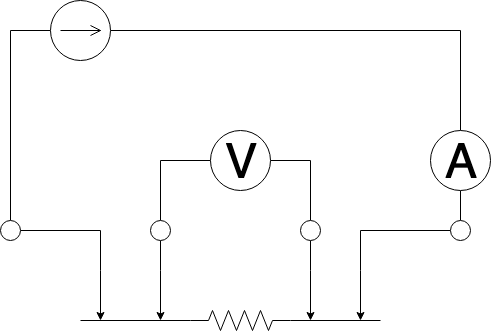
\includegraphics[width=60mm]{fig1.png}
  \end{center}
  \caption{ビームウエストと広がり角}
  \label{fig:one}
 \end{minipage}
 \begin{minipage}{0.45\hsize}
  \begin{center}
   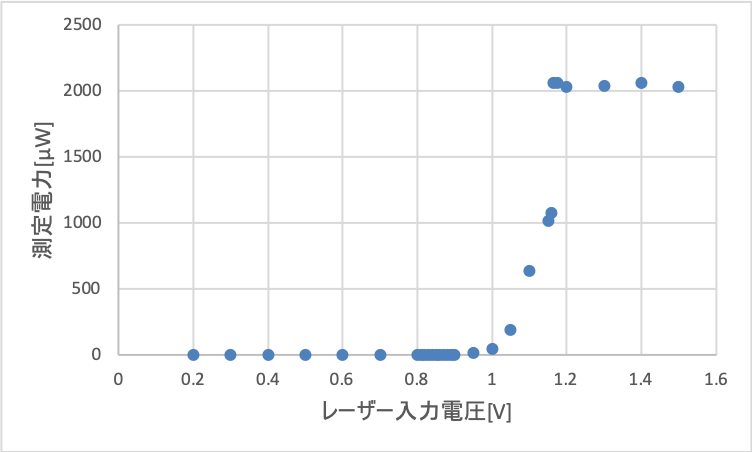
\includegraphics[width=60mm]{fig2.png}
  \end{center}
  \caption{$Distance$と$Diameter$}
  \label{fig:two}
 \end{minipage}
\end{figure}
\newpage
またこれらの距離、角度は下記の式(\ref{eq:a})の関係を満たす。
\begin{equation}
    d^2(z) = d_0^2 + \theta^2z^2 \label{eq:a}
\end{equation}\\
そのため$d_0$,$\theta$を求めるためには、スクリーンに映し出されたレーザーの直径の値、レーザーの射出口からスクリーンまでの距離、二つの測定値が必要となる。
ビーム半径を測定するためのスクリーンには方眼紙を用いた。
まず、スクリーンに当たったレーザー光の直径を方眼を用いて測定し$Diameter$を求めた。
次に、スクリーンまでの距離を物差しを用いて測定し$Distance$を求めた。




\subsubsection{Result}
測定結果から次の表が得られた。
\begin{table}[htb]
  \begin{center}
    \caption{レーザーからスクリーンの距離と直径}
    \begin{tabular}{rrr} \hline
        $Distance(mm)$ & $Diameter(mm)$  \\ \hline
        500            & 1.1 \\
        4000           & 5.0 \\ \hline
    \end{tabular}
    \label{tab:a}
  \end{center}
\end{table}


またこの測定結果より、関係式(\ref{eq:a})において変数消去を行うことで$d_0 = 0.915mm$, $\theta = 1.22 \times 10 ^{-3}rad$
という値が得られた。
この結果よりレーザー光は確かに射出口から遠ざかれば遠ざかるほど広がっていることが確認できた。
一方でレーザーの広がり角は上記の通り非常に小さい角度であることが確認できた。
\subsubsection{Discussion}
通常実験用レーザーの広がり角は($mrad$)オーダーであるので今回の実験結果は実際の広がり角から大きずれることなく測定できたと考えられる。
しかし測定精度を下げる要因として、ビーム直径を測定する際にビームの強度が強すぎたために目視の正確さを欠いたことや、観測者が毎回入れ替わったことによりそれぞれの直径の定義がバラバラであったことなどが挙げられる。

そもそもビームの光はガウス分布に従うため正確な境目が存在しない。
したがってガウスシアンビームのビーム半径はビーム軸の上のピーク値の$1/e^2$まで減少する半径と決められている。
つまりビームの$0.135$倍暗くなっている所を境界と定めるべきであった。

また、この測定から得られた$\theta$,$d_0$の値はレーザー特有の値であり測定地点の変化によって変わるものではないので$Distance$,$Diameter$を2回ずつしか計測すればそれぞれの値を推測することは可能である。
一方で、$Distance$,$Diameter$の測定回数を増やすことでよりビームウエストと広がり角の値をより正確に測定することができると考えられる。

さらに光の強度を下げてビーム半径を測定しやすくするためにNDフィルターを利用して測定を行うなどの改善策が挙げられる。
%=============================================================
\subsection{The Keplerian Beam Expander}
\subsubsection{Purpose}
レーザービームはそのままだと非常にビーム半径が小さく干渉現象を観察するときには不便である。
そのためビーム半径を広げるために二つのレンズを組み合わせてビームエキスパンダーを製作する必要がある。
今回の実験の目的はビームエキスパンダーの原理を理解し、今後行う光の干渉実験においてビームエキスパンダーを円滑に製作できるようになることである。
\subsubsection{Contents}
今回はケプラー型のビームエキスパンダーを製作する。
ケプラー型ビームエキスパンダーは凸レンズを二個組み合わせて製作する。
図(\ref{fig:three})に示すように光学系を組み立てた。
まずNDフィルター($1\%\times2,25\%$)3枚をレーザーの前に置き、次に焦点距離$50mm$の凸レンズ、さらに置焦点距離$200mm$の凸レンズを置いた。
次に二つ目のレンズを抜けた光が平行光となるようにレンズの位置を調整した。
さらにエキスパンダーの拡大率を計算するために一つ目のレンズを透過する前のビーム直径、二つ目のレンズを透過した後のビーム直径をそれぞれ計測し、実際の拡大率と理論値との比較を行った。
\begin{figure}[htbp]
 \begin{center}
  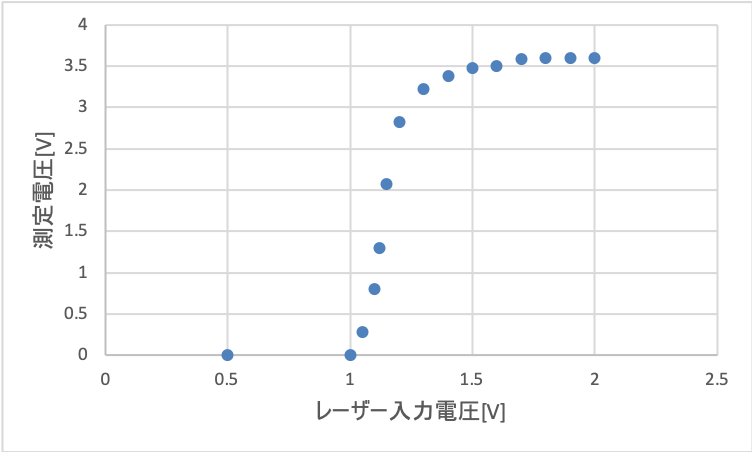
\includegraphics[width=100mm]{fig3.png}
 \end{center}
 \caption{ケプラー型ビームエキスパンダー}
 \label{fig:three}
\end{figure}

\subsubsection{Result}
二つ目のレンズを透過した光が平行光となったのはレンズ間距離$f_i + f_o$が$260mm$となった時であった。
またエキスパンダー入射前のビーム直径は$1.3mm$に対してエキスパンダーの透過光は$5.0mm$となりビームエキスパンダーを通ることでビーム半径が大きくなることが確認された。この時の拡大率は$3.85$であった。
\subsubsection{Discussion}
実験で使用した凸レンズは$f_i = 50mm$,$f_o = 200mm$だったので理論値としてはレンズ間の距離は$250mm$であるはずだが実験値はその値よりも大きい値となった。この理由としてはもともと凸レンズの焦点距離が異なっていた、ビームの軌跡がレンズの中心に当たっていなかった、などが考えられる。
また拡大率が理論値の4倍よりも小さく出てしまった原因についても上記と同様のことが考えられる。この場合拡大率が理論値よりも小さくなったので実際の二つのレンズの焦点距離は$f_i$が表示値よりも大きかったことが考えられる。そのように考えると平行光を作り出す時のレンズ間距離が理論値よりも大きくなってしまったことにも説明がつく。
%=============================================================
\subsection{The Galilean Beam Expander}
\subsubsection{Purpose}
今回はガリレオ型のビームエキスパンダーを製作する。
前述の通り干渉実験などビーム半径を広げたい時にビームエキスパンダーを用いる。
またガリレオ型のエキスパンダーはケプラー型よりも短い距離で高い倍率を実現できる。
\subsubsection{Contents}
図(\ref{fig:three})に示すように工学系を組み立てた。
まず前回同様、NDフィルター($1\%\times2,25\%$)3枚をレーザーの前に置いた。
次に焦点距離$-40mm$の凹レンズを置き、その後で前回使用した焦点距離$200mm$の凸レンズを置いた。
次にエキスパンダーの透過光が平行光となるようにレンズ間の距離を調節した。
またエキスパンダーの透過光のビーム直径を測定し、透過前のビームと直径と比べて拡大率を計算し、理論値をの違いを比べた。
\begin{figure}[htbp]
 \begin{center}
  \includegraphics[width=100mm]{fig4.png}
 \end{center}
 \caption{ガリレオ型ビームエキスパンダー}
 \label{fig:four}
\end{figure}
\subsubsection{Result}
エキスパンダーの透過光が平行光になる時のレンズ間の距離は$160mm$であり理論値と一致した。
また、エキスパンダー透過前のビーム直径は$1.5mm$であったのに対して、エキスパンダーを通った後のビーム直径は$7.5mm$であった。
以上より実験での拡大率は$5.0$でありこれも理論値と一致した。
\subsubsection{Discussion}
今回の実験ではレンズ間距離もエキスパンダーの倍率も理論値と一致した。
しかし観測者を前の実験から入れ替えてしまったのでケプラー型の時と比べビーム直径の測り方に若干のズレが生じてしまった。
またケプラー型、ガウス型のエキスパンダーの実験を通してどちらのエキスパンダーもレンズ間距離は$f_i + f_o$で与えられるが、ガウス型の方が凹レンズを使用しているため$f_i$の焦点距離が負になるため同じ拡大率を実現しようとするとガウス型の方がより短いレンズ間距離で実現することができる。
またガウス型はエキスパンダーを通る前と後で像が逆転しないという利点もある。
これらのエキスパンダーの応用例としてはプロジェクションマッピングなどで拡大した大きい像を見せたい時に応用することができる。
%=============================================================
%=============================================================

\section{Diffraction from circular apertures and slits}
\subsection{Circular aperture}
\subsubsection{Purpose}
今回の実験では、円形開口による干渉縞パターンを観測する。
また干渉縞の間隔から円形開口の直径を推測する。
また円形開口を顕微鏡により長さを測定することで実験値とのさを比較する。
\subsubsection{Contents}
図(\ref{fig:five})に示すように光学系を組み立てた。
またそれぞれの距離を図(\ref{fig:five})に示すよに名前をつけた。
まず、レーザーの前に円形開口を置きそこから離れた距離にスクリーンを設置した。
今回は$02mm$,$0.4mm$の二つの円形開口を用いて実験を行なった。
また、スクリーンは方眼紙で製作した。
次に開口からクリーンまでの距離$L$を測定した。
レーザーの電源をつけるとスクリーンに円形の干渉縞が得られた。
円形の干渉縞の中心から1番目の暗線のまでの距離$r$を測定した。
これを二種類の円形開口に対して距離$L$を変えながら二回ずつ計測を行なった。
\begin{figure}[htbp]
 \begin{center}
  \includegraphics[width=100mm]{fig5.png}
 \end{center}
 \caption{円形開口の光学系}
 \label{fig:five}
\end{figure}\\

またこれらの測定した距離は式(\ref{eq:b})の関係をみたす。
\begin{equation}
    sin\theta = \frac{1.22\lambda}{D} \label{eq:b}
\end{equation}\\


またこの時$\theta$,$D$の値は非常に小さいので$sin\theta \simeq tan\theta = r/L$とみなすことができる。
また今回使用したHe-Ne Laserの波長は$\lambda = 632.8nm$である。
以上より計測値を関係式へ代入して円形開口の直径を推測した。
\subsubsection{Result}
測定結果から次の表が得られた。
\begin{table}[htb]
 \begin{minipage}{0.45\hsize}
  \begin{center}
    \caption{$0.2mm$円形開口}
    \begin{tabular}{rrr} \hline
        $r(mm)$ & $L(mm)$ & $D(mm)$  \\ \hline
        0.25     & 583 & 0.18\\
        0.45    & 1435 & 0.246\\ \hline
    \end{tabular}
    \label{tab:b}
  \end{center}
 \end{minipage}
 \begin{minipage}{0.45\hsize}
  \begin{center}
    \caption{$0.4mm$円形開口}
    \begin{tabular}{rrr} \hline
        $r(mm)$ & $L(mm)$ & $D(mm)$  \\ \hline
        2.6   & 974 & 0.289\\
        3.5    & 1430 & 0.315\\ \hline
    \end{tabular}
    \label{tab:c}
  \end{center}
 \end{minipage}
\end{table} 
\newpage


またそれぞれ以下のような干渉模様が観測できた。
\begin{figure}[htbp]
 \begin{minipage}{0.45\hsize}
  \begin{center}
   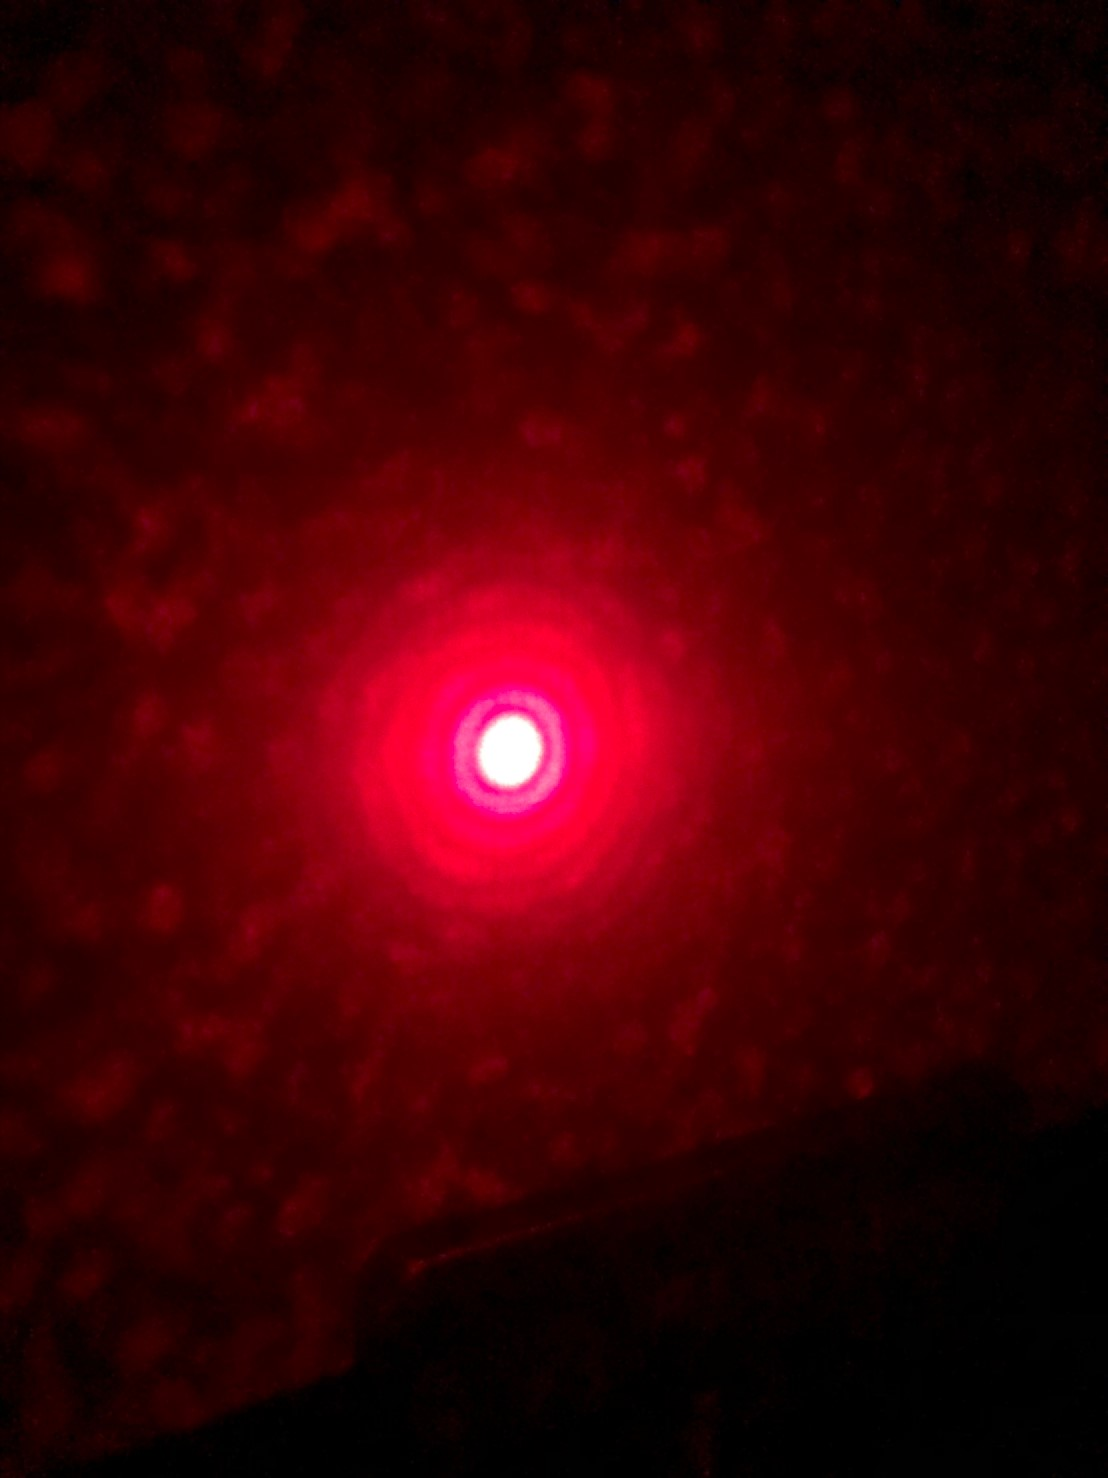
\includegraphics[width=60mm]{fig6.png}
  \end{center}
  \caption{$0.2m$円形開口の干渉縞}
  \label{fig:six}
 \end{minipage}
 \begin{minipage}{0.45\hsize}
  \begin{center}
   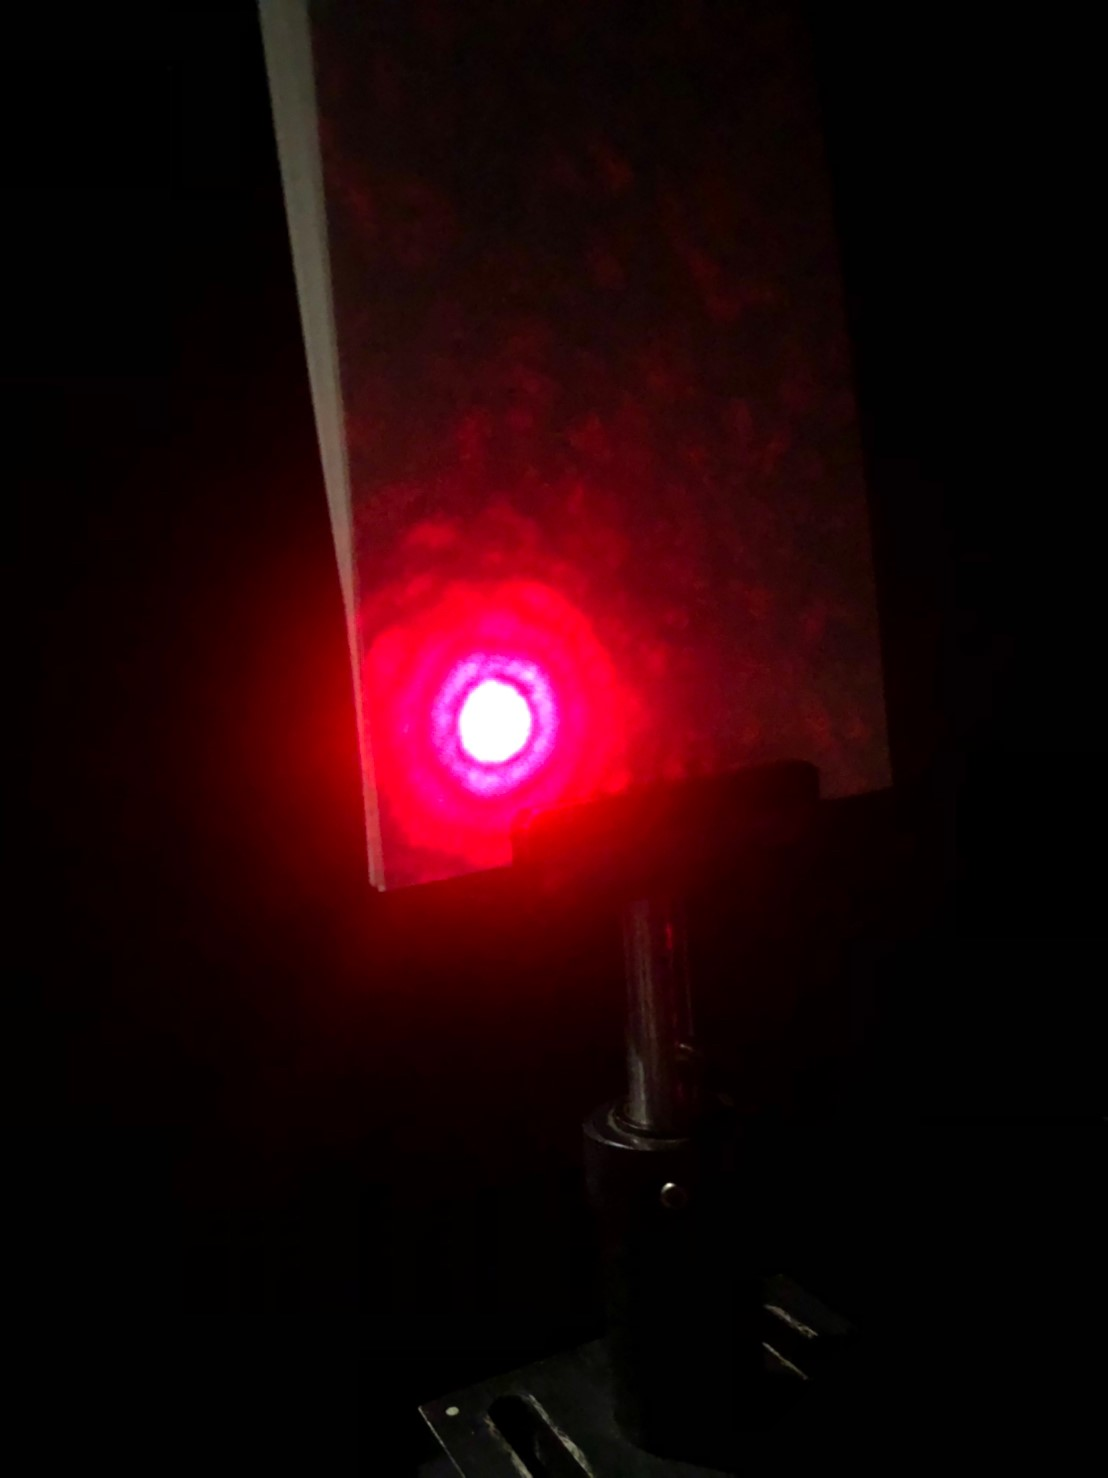
\includegraphics[width=60mm]{fig7.png}
  \end{center}
  \caption{$0.4m$円形開口の干渉縞}
  \label{fig:seven}
 \end{minipage}
\end{figure}


干渉模様は円の半径が大きくなっていく連れて明暗の境目が不明瞭になって区別がつかなくなった。
\subsubsection{Discussion}
$0.2mm$円形開口の実験値と理論値の差は比較的小さかった。一方で$0.4mm$円形開口の理論値との差はかなりの開きがあった。
これは円形開口の円がそもそも真円ではなく大きさ自体の制度もまちまちであった可能性が考えられる。
さらに他の要因としてそもそも$D$を算出する際に$sin\theta \simeq tan\theta = r/L$と近似したために実際の値とは異なる結果となった可能性が考えられる。
さらには目測による測定に誤差があったなどの要因も考えられる。
また干渉には開口部の大きさがスクリーンまでの距離に対して十分小さい時に起こるフレネル回折、ビーム源もしくは観測点がビームを回折するものから無限遠に位置する時に起こるフラウンホーファー回折などがあるが今回の実験での回折はフレネル回折であることが考えられる。
%=============================================================
\subsection{Single Slit}
\subsubsection{Purpose}
今回はシングルスリットの干渉縞を観測する。
前回の円形開口の干渉縞との違いを観察して、スクリーンからの距離、明線暗線の間隔を測る事によりスリット幅を算出することが目的である。
\subsubsection{Contents}
基本的には前回と同じ光学系を組み立てる。
今回は円形開口の代わりにシングルスリットをレーザーの前に置いた。
以下の図はシングルスリットの光学系である。
今回は$r$,$L$の距離を測定する事によって$\omega$の値を推測する。
またこの実験では$0.1mm$,$0.2mm$二つのスリットを用いてそれぞれ1回ずつ測定を行なった。
\begin{figure}[htbp]
 \begin{center}
  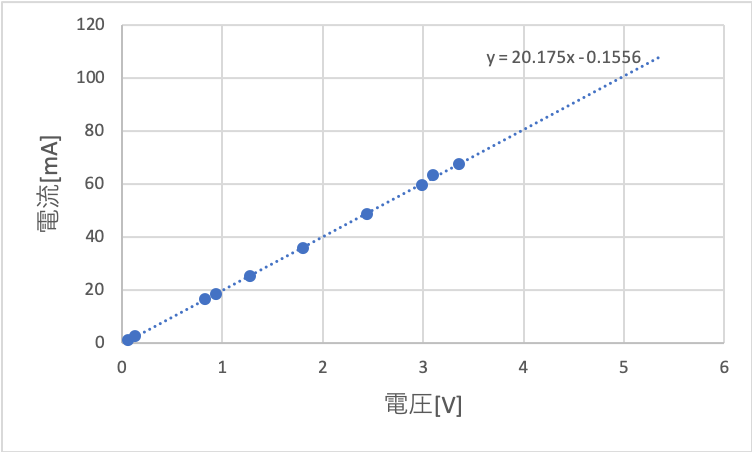
\includegraphics[width=100mm]{fig8.png}
 \end{center}
 \caption{シングルスリットの光学系}
 \label{fig:eight}
\end{figure}\\

またこれらの測定した距離は
\begin{equation}
    sin\theta = \frac{\lambda}{\omega} \label{eq:c}
\end{equation}\\
式(\ref{eq:c})の関係をみたす。
またこの時$\theta$,$D$の値は非常に小さいので$sin\theta \simeq tan\theta = r/L$とみなすことができる。
また今回使用したHe-Ne Laserの波長は$\lambda = 632.8nm$である。
以上より計測値を関係式へ代入してシングルスリットの間隔を推測した。

\subsubsection{Result}
測定結果から次の表が得られた。\\
\begin{table}[htb]
 \begin{minipage}{0.45\hsize}
  \begin{center}
    \caption{$0.1mm$シングルスリット}
    \begin{tabular}{rrr} \hline
        $r(mm)$ & $L(mm)$ & $\omega(mm)$  \\ \hline
        7.0    & 974 & 0.088\\ \hline
    \end{tabular}
    \label{tab:d}
  \end{center}
 \end{minipage}
 \begin{minipage}{0.45\hsize}
  \begin{center}
    \caption{$0.2mm$シングルスリット}
    \begin{tabular}{rrr} \hline
        $r(mm)$ & $L(mm)$ & $\omega(mm)$  \\ \hline
        3.5    & 974 & 0.176\\ \hline
    \end{tabular}
    \label{tab:e}
  \end{center}
 \end{minipage}
\end{table}

またそれぞれ以下のような干渉模様が観測できた。\\
\begin{figure}[htbp]
 \begin{minipage}{0.45\hsize}
  \begin{center}
   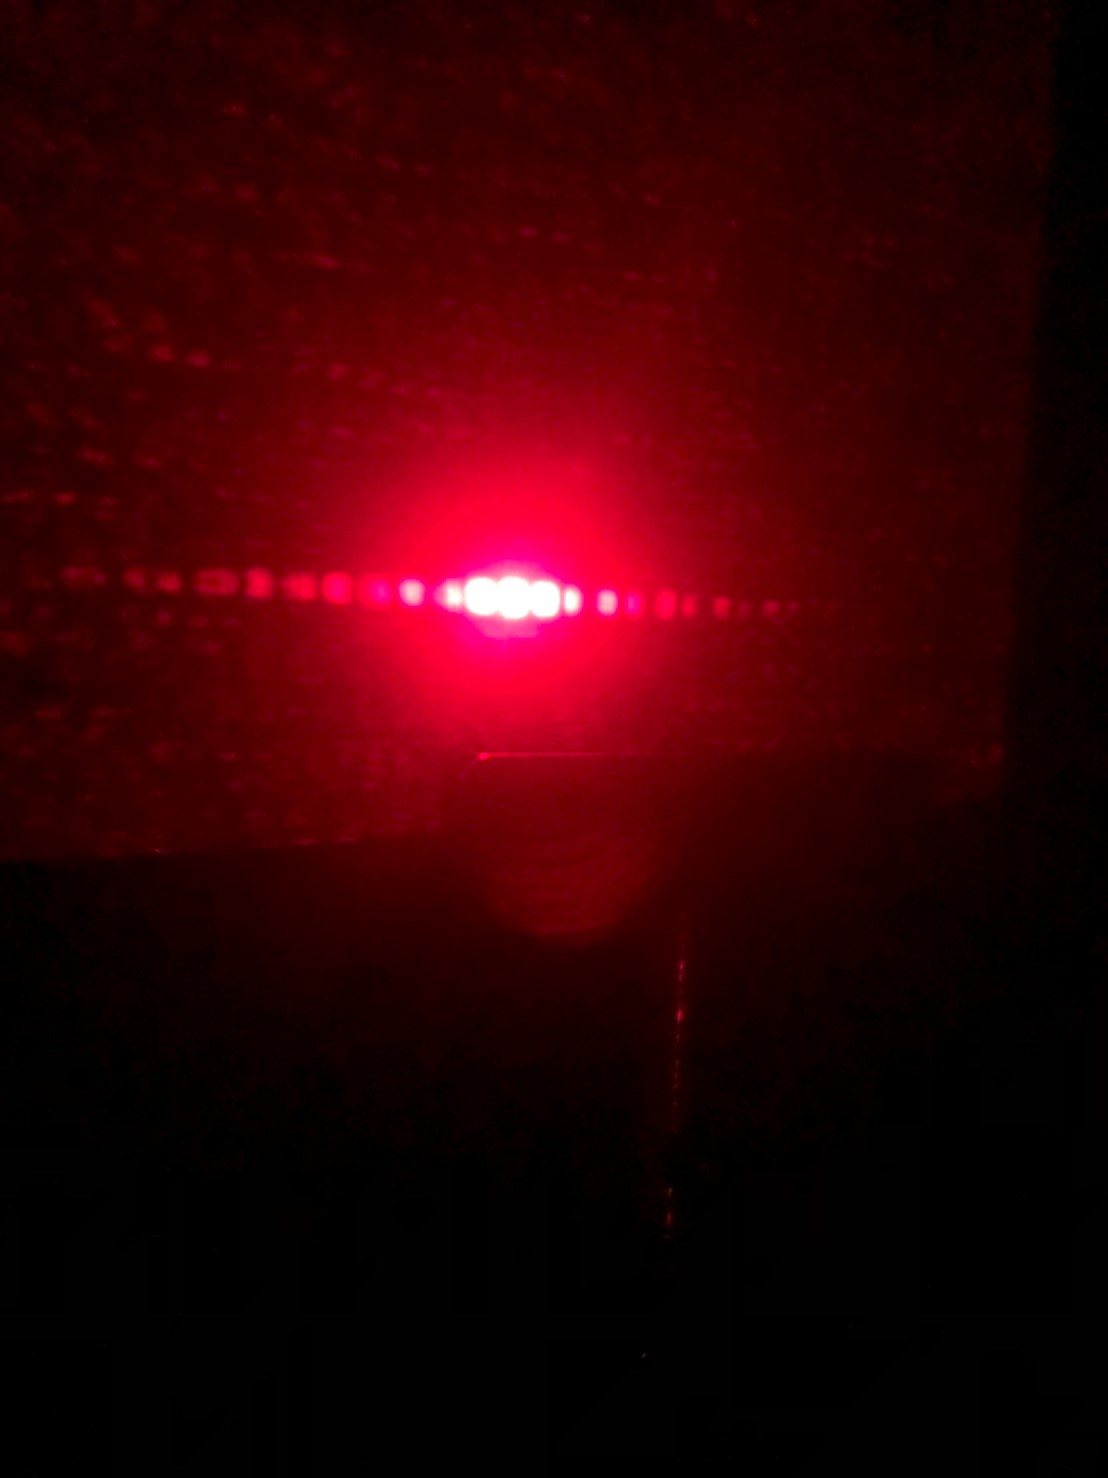
\includegraphics[width=60mm]{fig9.png}
  \end{center}
  \caption{$0.1m$シングルスリットの干渉縞}
  \label{fig:nine}
 \end{minipage}
 \begin{minipage}{0.45\hsize}
  \begin{center}
   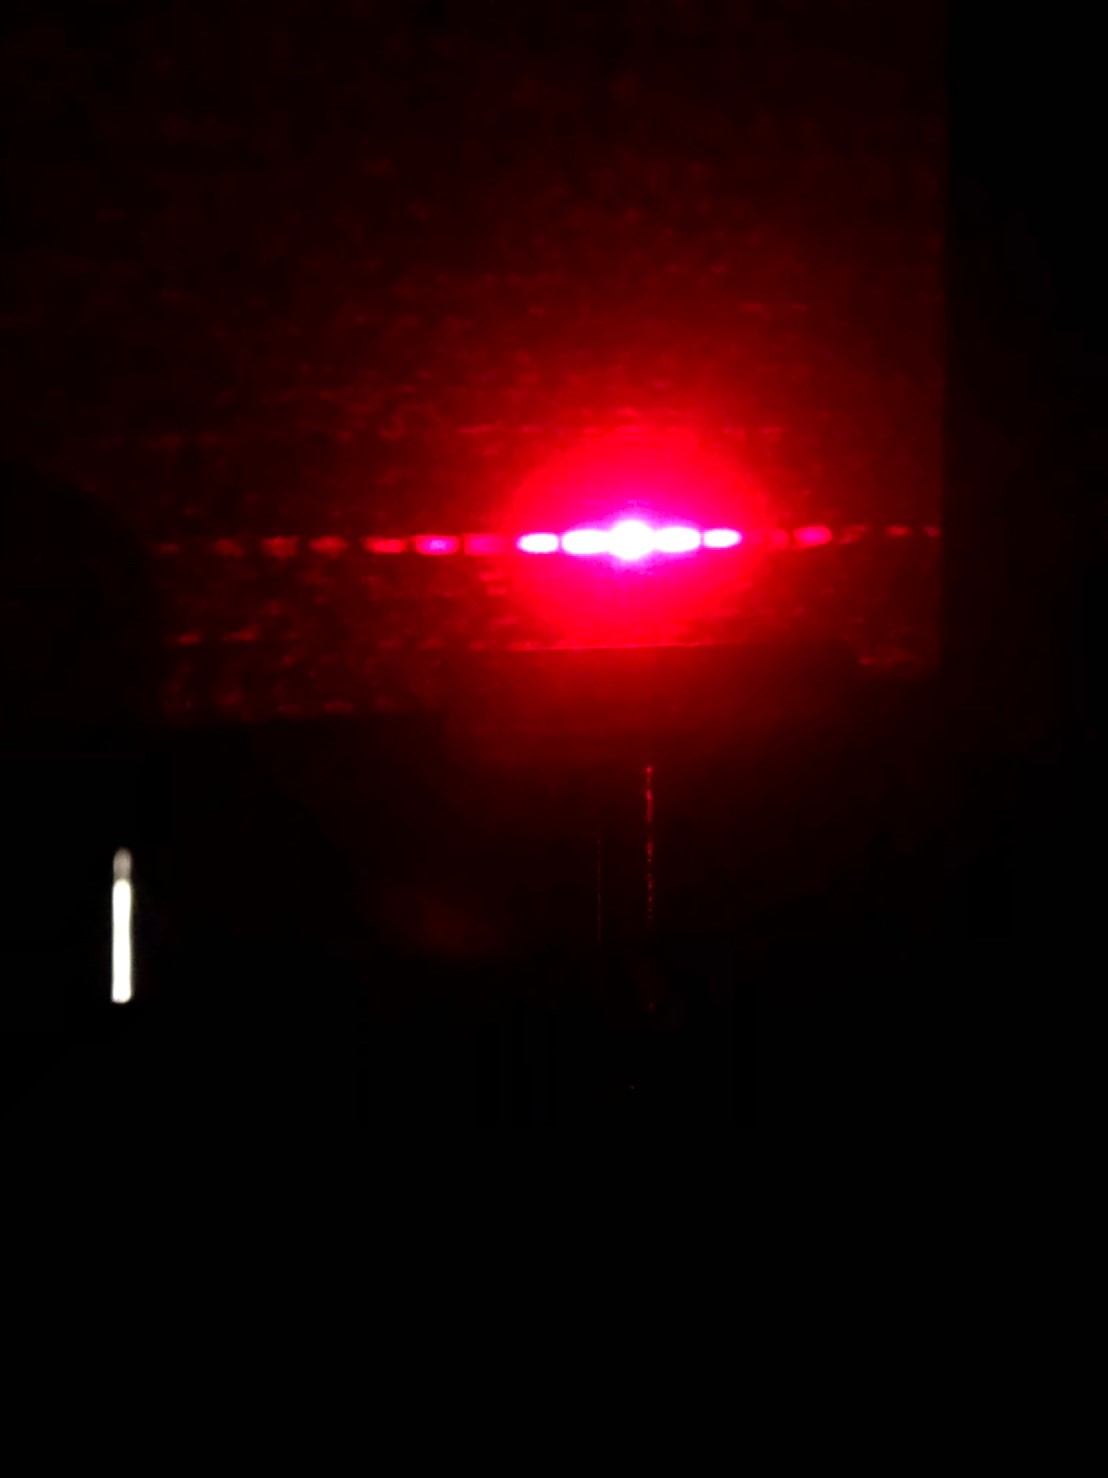
\includegraphics[width=60mm]{fig10.png}
  \end{center}
  \caption{$0.2m$シングルスリットの干渉縞}
  \label{fig:ten}
 \end{minipage}
\end{figure}
\subsubsection{Discussion}
式(\ref{eq:c})の関係よりスリット幅が大きくなるにつれて干渉縞の間隔は小さくなっていく。実験からもこの関係が確かめられた。
いずれの結果も理論値よりも$0.02mm$ほど小さくなってしまったのでどちらも目測による計測の時実際の感覚よりも大きく読んでしまった可能性が考えられる。
%=============================================================
\subsection{Yong Double Slit}
\subsubsection{Purpose}
今回はヤングのダブルスリットによる干渉縞を観測する。
前回のシングルスリットとどう違った干渉をするのかを理解するのが目的である。
\subsubsection{Contents}
光学系を図(\ref{fig:eleven})に示すように製作した。
ダブルスリットをビームの経路に置きビーム光を回折させスクリーンに干渉縞を映し観察した。

\begin{figure}[htbp]
 \begin{center}
  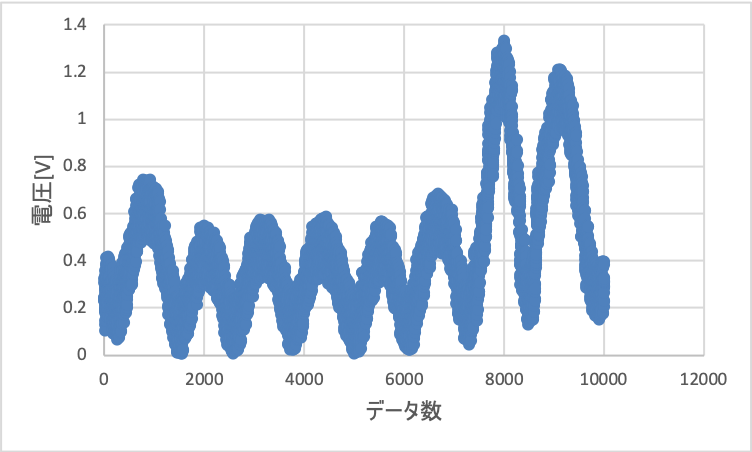
\includegraphics[width=100mm]{fig11.png}
 \end{center}
 \caption{ダブルスリットの光学系}
 \label{fig:eleven}
\end{figure}

またこの時以下の式(\ref{eq:d}),(\ref{eq:f})の関係が成り立つ。それぞれ測定した$\Delta \theta$,$\Delta x$を式に代入することで二つのスリット幅$d$
を推測した。
また今回は$0.2mm$,$0.1mm$の二つのスリット間隔をを持つダブルスリットに対して一回ずつ計測を行なった。\\
\begin{equation}
    \Delta\theta = \frac{\Delta x}{R} \label{eq:d}
\end{equation}\\
\begin{equation}
    \Delta\theta = \frac{\lambda}{d} \label{eq:f}
\end{equation}\\

\subsubsection{Result}
測定結果から次の表が得られた。

\begin{table}[htb]
 \begin{minipage}{0.45\hsize}
  \begin{center}
    \caption{$0.1mm$ダブルスリット}
    \begin{tabular}{rrr} \hline
        $\Delta x(mm)$ & $R(mm)$ & $d(mm)$  \\ \hline
        7.0    & 974 & 0.088\\ \hline
    \end{tabular}
    \label{tab:f}
  \end{center}
 \end{minipage}
 \begin{minipage}{0.45\hsize}
  \begin{center}
    \caption{$0.2mm$ダブルスリット}
    \begin{tabular}{rrr} \hline
        $\Delta x(mm)$ & $R(mm)$ & $d(mm)$  \\ \hline
        2.8    & 974 & 0.22\\ \hline
    \end{tabular}
    \label{tab:g}
  \end{center}
 \end{minipage}
\end{table}
\newpage
また以下のような干渉縞が観察された。

\begin{figure}[htbp]
 \begin{minipage}{0.45\hsize}
  \begin{center}
   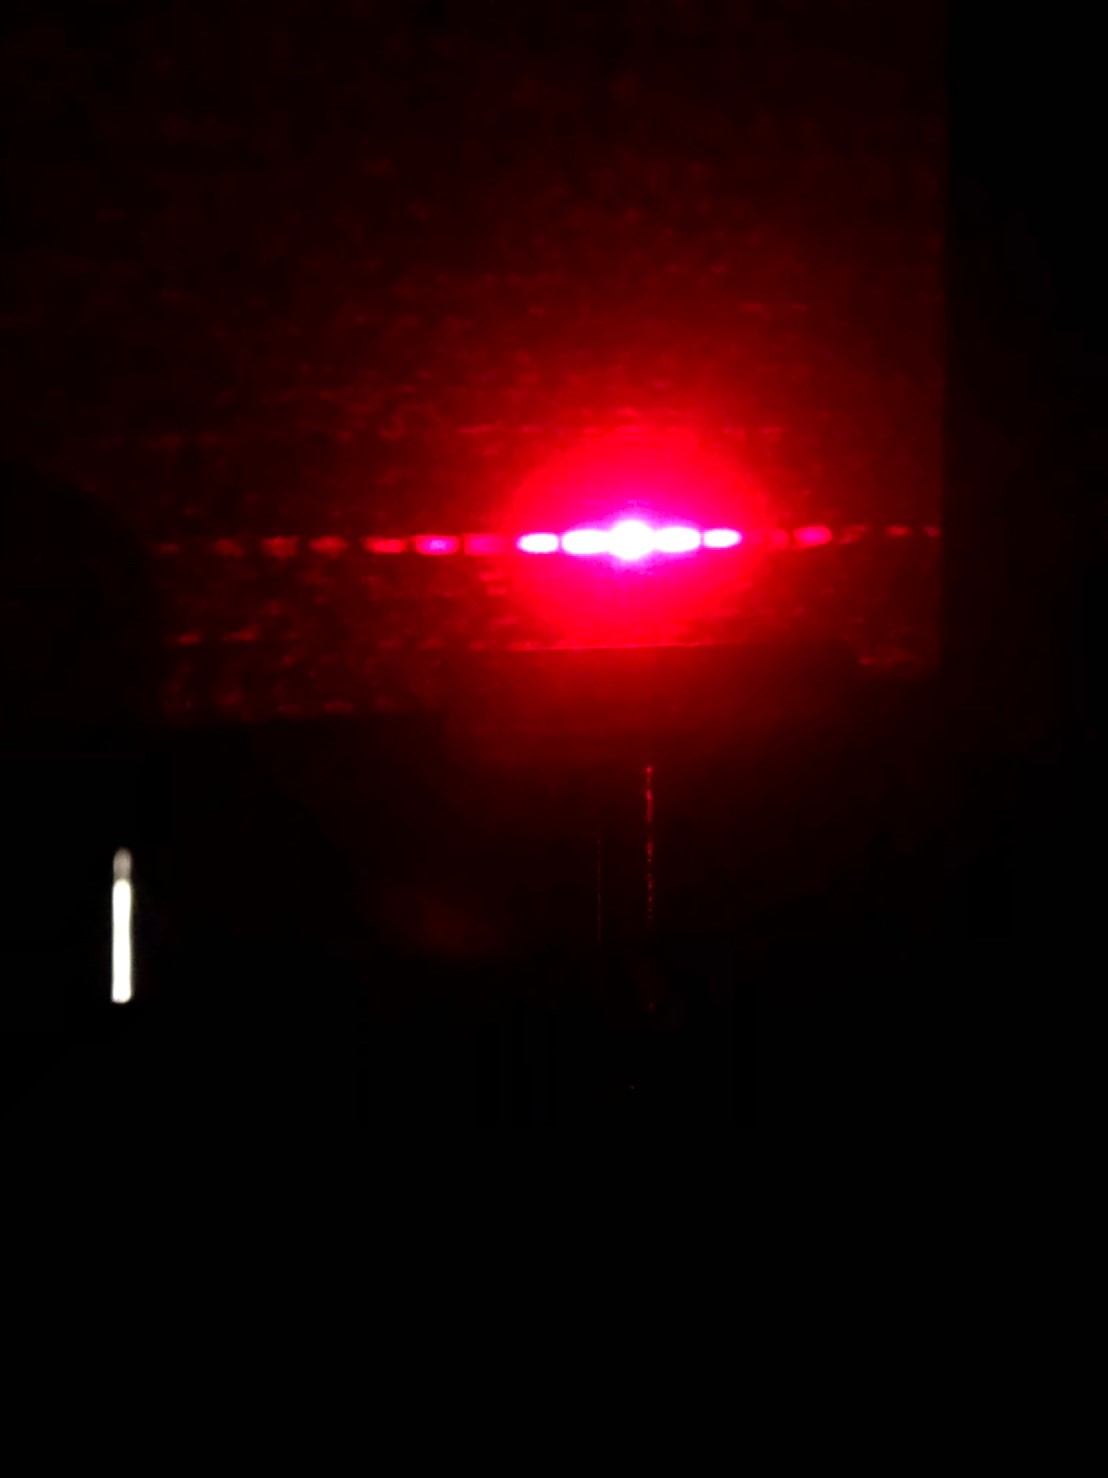
\includegraphics[width=60mm]{fig12.png}
  \end{center}
  \caption{$0.1m$ダブルスリットの干渉縞}
  \label{fig:12}
 \end{minipage}
 \begin{minipage}{0.45\hsize}
  \begin{center}
   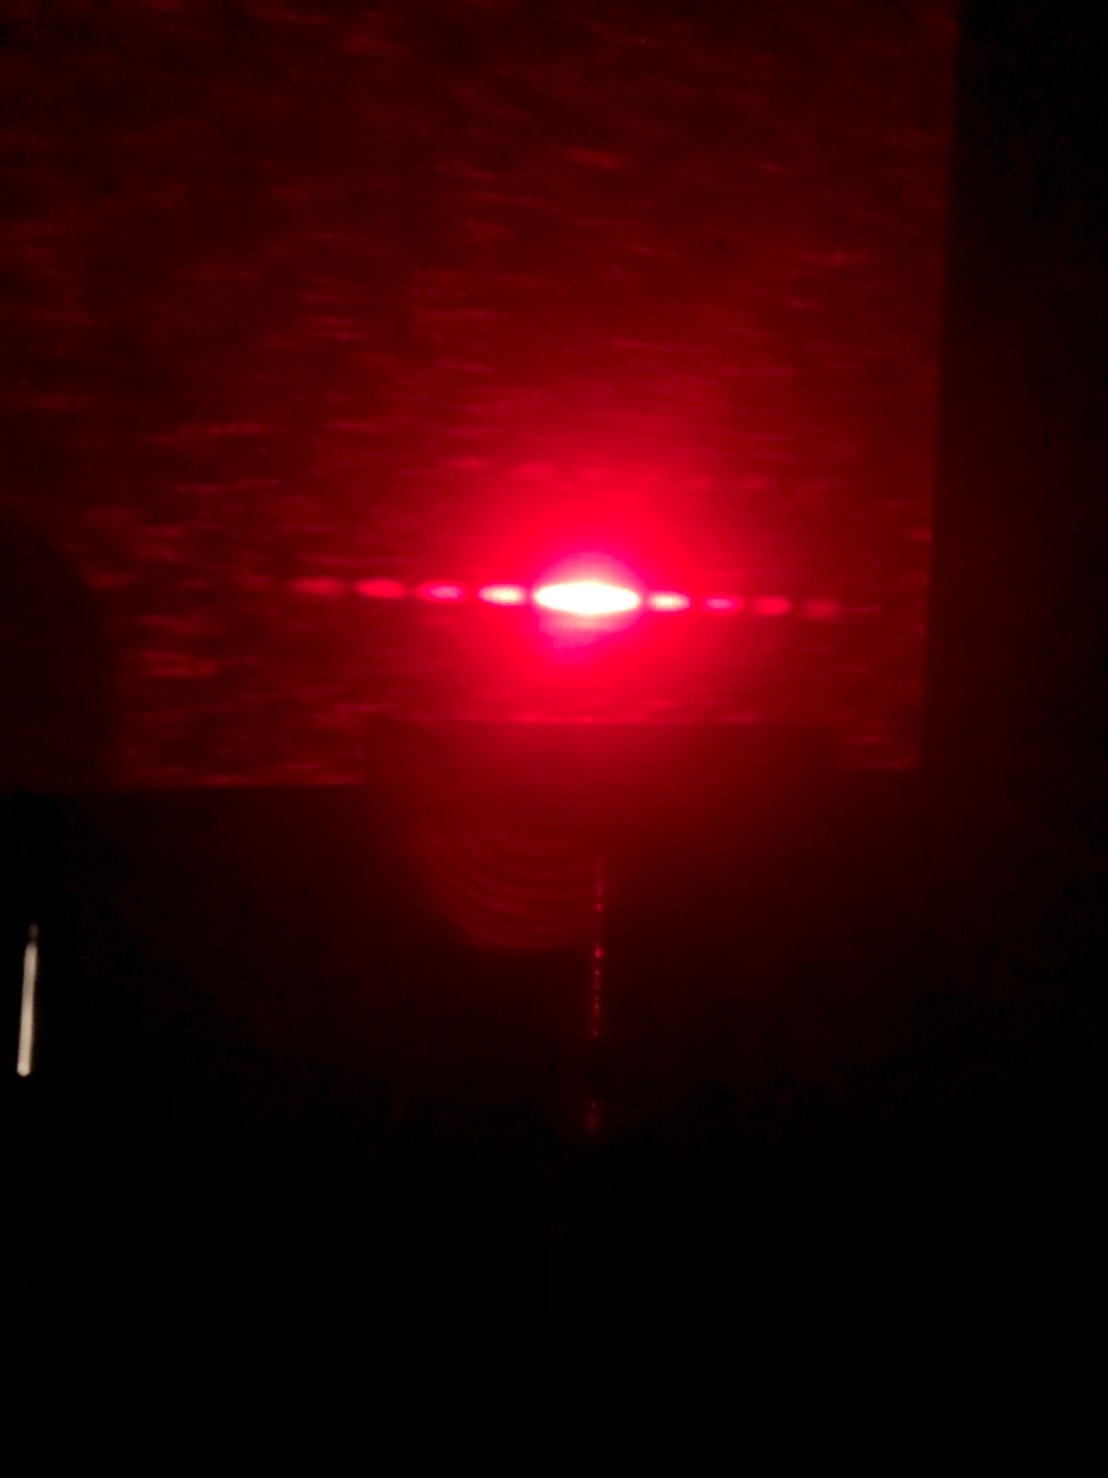
\includegraphics[width=60mm]{fig13.png}
  \end{center}
  \caption{$0.2m$ダブルスリットの干渉縞}
  \label{fig:13}
 \end{minipage}
\end{figure}

\subsubsection{Discussion}
どちらの誤差も$-0.02mm$であったので目測の際に$r$を大きく読んでしまったことなどが考えられる。
またシングルスリットの時と同じような干渉縞が得られたがシングルスリットの方が中心が明るく、ダブルスリットの時は中心から離れた干渉縞でも強度が高かったことが観測された。これはダブルスリットの際は二つのスリットを通過した際にビーム光が素元波となり互いの波が干渉をするためだと考えられる。

%=============================================================
%==============================================================
\section{Michelson Interferometer and Coherence}
\subsection{Michelson Interferometer}
\subsubsection{Purpose}
今回の実験では二つのビーム光をハーフミラーで分けた後再び合流した光で干渉縞を作り出すのが目的である。
また干渉を作り出すためハーフミラーやミラービームエキスパンダーなどを適切に組み立て配置することも重要である。
\subsubsection{Contents}
まず以下のように干渉計を組み立てる。
\begin{figure}[htbp]
 \begin{center}
  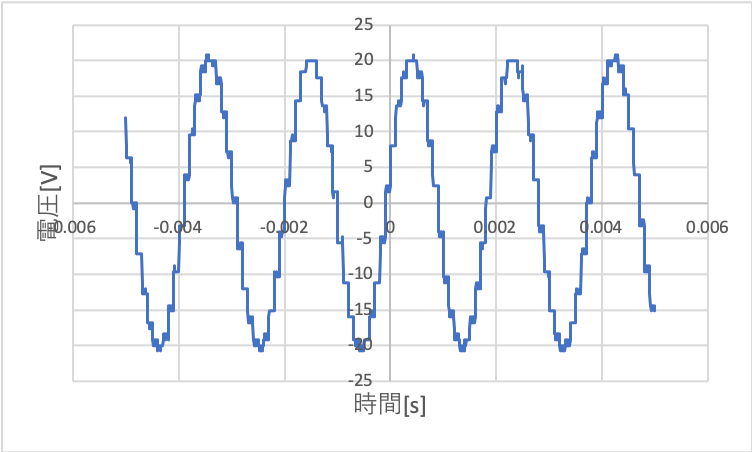
\includegraphics[width=100mm]{fig14.png}
 \end{center}
 \caption{マイケルソン干渉計}
 \label{fig:14}
\end{figure}\\

まず光の強度を弱めるためにNDフィルター(25\%)をレーザーの前に設置した。
次にビームエキスパンダーを組み立てた。今回はガリレオ型のエキスパンダーを組み立てた。
また、それぞれのミラーの高さを合わせて跳ね返った光がスクリーン上で一致するように調整を行なった。
次にM2のミラーを移動させることで干渉縞が観測されたので干渉模様を写真におさめた。
さらにその状態から机を叩く事により干渉模様がどのように変化するかを観察した。
その後エキスパンダーの二個目の凸レンズを移動させて二つのレンズ間距離を小さくする事で干渉模様にどのような変化が起きたかを観察した。
得られた干渉縞の写真をカメラにおさめた。
またこの時$BS-M1 = 8.0cm$,$BS-M2 = 5.0cm$の距離であった。

\subsubsection{Result}
二つの光がスクリーン上で重なり干渉を起こす事で図(\ref{fig:15})のような干渉模様が得られた。
また机を叩いて揺れを起こす事でスクリーン上に映っていた干渉模様が消えた。
その後0.98[s]後に元どおりの干渉模様をまた形成した。
さらにエキスパンダーのレンズ間距離を小さくすると干渉模様が図(\ref{fig:16})のように円の一部分のように丸くなって映った。
さらにレンズ間距離を元の位置よりも大きくすると同じような円状の干渉模様が得られた。
\newpage

\begin{figure}[htbp]
 \begin{minipage}{0.45\hsize}
  \begin{center}
   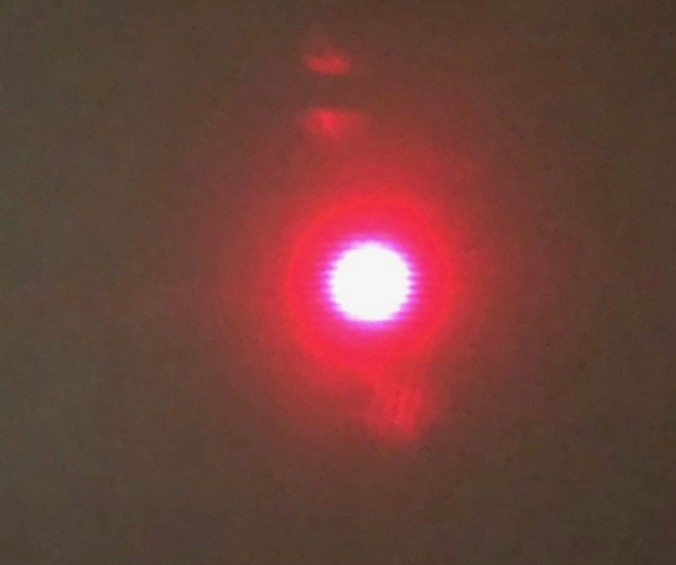
\includegraphics[width=60mm]{fig15.png}
  \end{center}
  \caption{干渉模様}
  \label{fig:15}
 \end{minipage}
 \begin{minipage}{0.45\hsize}
  \begin{center}
   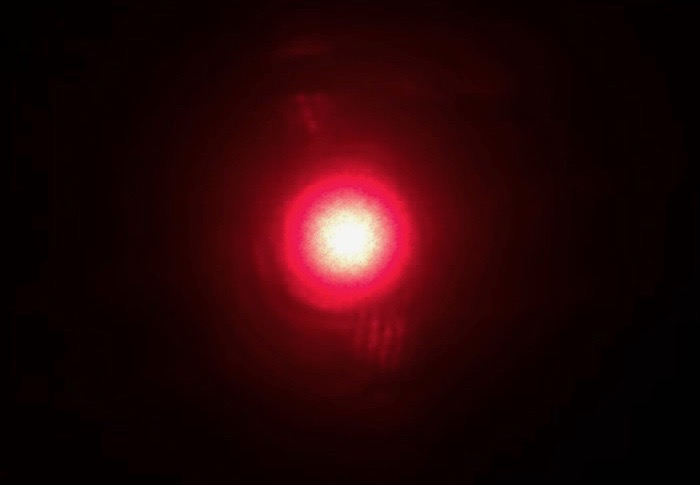
\includegraphics[width=60mm]{fig16.png}
  \end{center}
  \caption{レンズ間を狭くした時の干渉模様}
  \label{fig:16}
 \end{minipage}
\end{figure}

\subsubsection{Discussion}
まずM2の位置を調節する事でスクリーン上に平行な干渉模様が得られたからM1に反射された光とM2に反射された光がそれぞれ平面波であってその波がスクリーン上でぶつかる事によって干渉模様が得られたと考えられる。
この事実から実験で使用したレーザーはコヒーレントな光であると言える。

また机を叩いた際に干渉模様が見えなくなったのは叩いた振動によってビーム光がコヒーレンスを失って位相が揃わなくなったからだと考えられる。

さらにエキスパンダーのレンズ間距離を縮めた際に同心円状の干渉模様が得られたのは平行光だったビーム光が球面はになった為だと考えられる。


%=============================================================
\subsection{Coherence}
\subsubsection{Purpose}
前回の実験よりビーム光がコヒーレンスな光だと確認できたが今回の実験では、光路差がどの程度まで離れるとコヒーレンスを失うのか(コヒーレント長)を計測する。
\subsubsection{Contents}
前回の実験と同様に図(\ref{fig:14})の光学系を製作する。初めの$BS-M1 = 8.0cm$,$BS-M2 = 5.0cm$の状態から$BS-M1$の距離のみを次第に広げていきスクリーン状で干渉模様が得られなくなるまで広げていきコヒーレント長を決定する。
\subsubsection{Result}
$BS-M1 = 10.0cm$の時は干渉模様が観測された。しかし$BS-M1 = 12.5cm$にすると干渉模様は見れなくなった。
以上の結果より可干渉光路差は$(|BS-M1|-|BS-M2|) \times 2 = 4.0cm$である事がわかった。
\subsubsection{Discussion}
一般のビーム光のコヒーレント長は10cm前後であるので今回の実験から得られた値とは大きな開きがあった。
この原因としては二つの光の交差する角度が小さかったために干渉模様が得られなかった、調節不足で本当はあったのに観測できなかったなどの理由が考えられる。

%=============================================================
%=============================================================
\section{Polarization of Light}
\subsection{Law of Malus}
\subsubsection{Purpose}
今回の実験ではフォトディテクターを用いて偏光によってレーザー光の強度がどのように変化するのかを確認する。
\subsubsection{Contents}
光学系を図(\ref{fig:17})のように製作する。
今回はNDフィルターは用いなかった。
まずビーム光の光路に二つの偏光板P1,P2を挿入する。
次に偏光された光がフォトディテクターの中心に来るように調整する。
初めに二つの偏光板の偏光角をどちらも同じに揃える。
その後10°ずつP2の角度を変えていきながらフォトディテクターに検出される偏光光の強度を観測してグラフにその推移をプロットしていく。

\begin{figure}[htbp]
 \begin{center}
  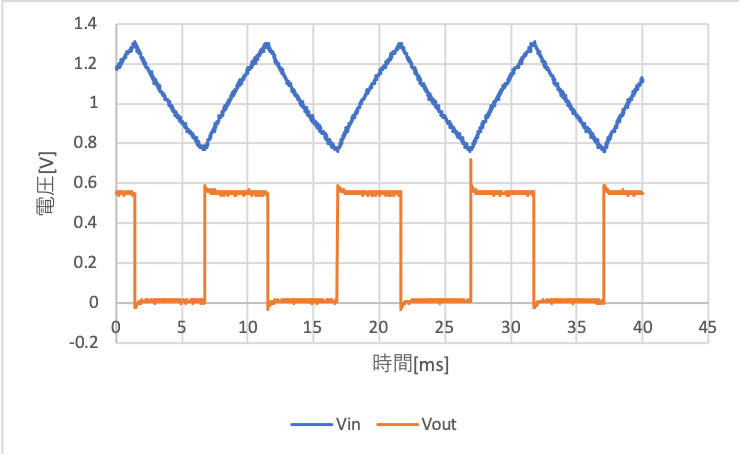
\includegraphics[width=100mm]{fig17.png}
 \end{center}
 \caption{偏光実験の光学系}
 \label{fig:17}
\end{figure}

\subsubsection{Result}
実験より得られた結果をプロットした図を下に示す。

\begin{figure}[htbp]
 \begin{center}
  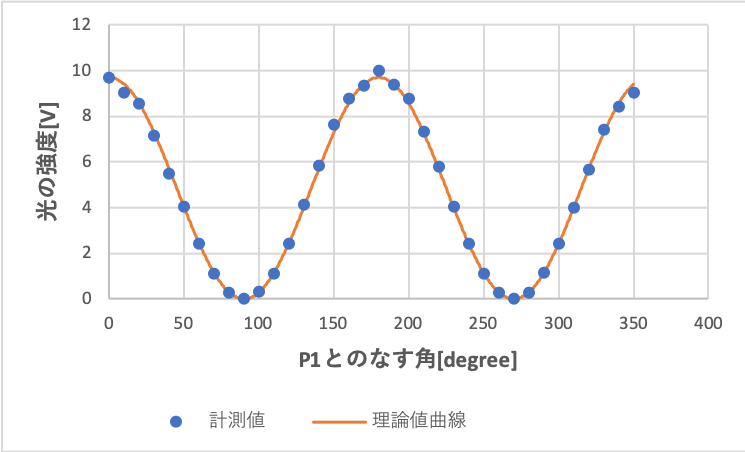
\includegraphics[width=100mm]{fig18.png}
 \end{center}
 \caption{偏光角と光の強度の強さ}
 \label{fig:18}
\end{figure}

実験結果から得られたグラフよりP1となす角を$\theta$、光の強度を$I$、偏光角0°の時の光の強度を$I_0$とした時にこのグラフの概形は以下の式のようになった。

\begin{equation}
    I = I_0cos^2\theta \label{eq:g}
\end{equation}\\
\subsubsection{Discussion}
グラフのように光の強度が変化したのはP1で偏光されて向きが統一されたビーム光をさらにP2で偏光するためP1,P2が垂直に近くなる程、偏光後の光の強度は小さくなっていくためであると考えられる。
また強度が$cos^2\theta$に比例する理由は、まずP2で偏光されることで波振幅はその余弦成分のみが取り出されるため、結果として強度は振幅の二乗に比例するので$cos^2\theta$に比例する結果となると考えられる。
%=============================================================
\subsection{Reflection}
\subsubsection{Purpose}
今回の実験では偏光された光の反射波の強度について調べる。
入射面に垂直なS偏光光と平行なP偏光光とで反射光の強度に違いが生じるのかを調べる。
またP偏光に関しては反射率が0となる角度、ブリュースター角の測定を行う
\subsubsection{Contents}
図(\ref{fig:19})のように光学系を製作する。
まず入射面に対し垂直に振幅するS偏光、入射面に対して平行に振幅するP偏光の二つの光を偏光板を使って作り出す。この時二つの偏光光の強度を等しくするためにビームの振幅は入射面に対して45°をなすように設置する。
次に偏光光をスライドガラス(屈折率 n = 1.52)に当てて反射させた。
この際スライドガラスにオイルをつけてプリズムに固定した。
その後二つの偏光光ごとに反射光の強度をフォトディテクターを用いて計測した。
反射角は10°から10°刻みに大きくしていき60°まで測定した。
特にP偏光に関してはブリュースター角付近の55°前後を2°ずつ測定した。
測定後に入射角と反射光の強度の関係をグラフにプロットした。
またブリュースター角は相対屈折率nとすれば式(\ref{eq:g})で与えられる。

\begin{equation}
    \theta_B = arctan(n) \label{eq:h}
\end{equation}\\

\begin{figure}[htbp]
 \begin{center}
  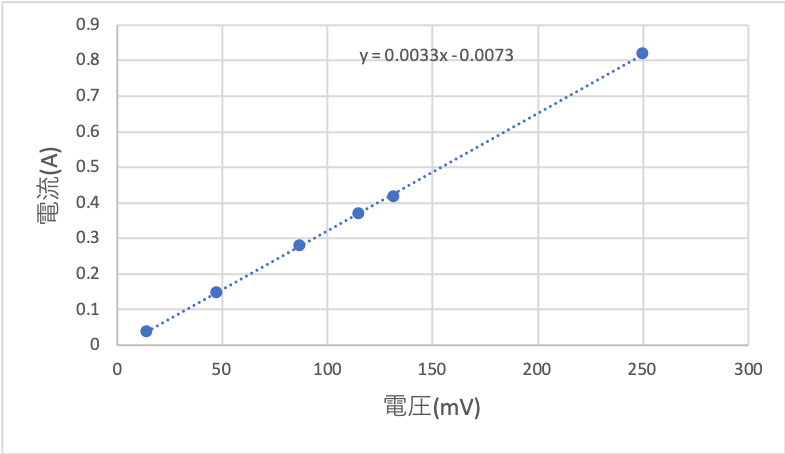
\includegraphics[width=100mm]{fig19.png}
 \end{center}
 \caption{反射強度の実験}
 \label{fig:19}
\end{figure}

\subsubsection{Result}
結果をグラフにプロットすると以下のようになった。

\begin{figure}[htbp]
 \begin{minipage}{0.45\hsize}
  \begin{center}
   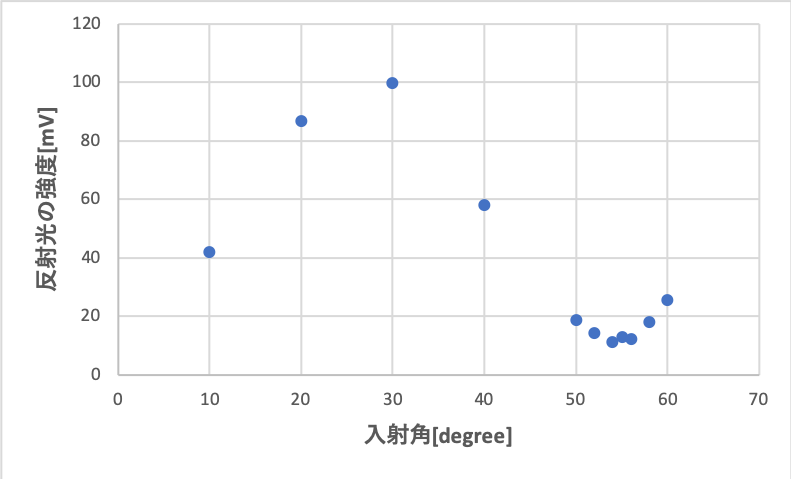
\includegraphics[width=60mm]{fig20.png}
  \end{center}
  \caption{P偏光の反射光強度}
  \label{fig:20}
 \end{minipage}
 \begin{minipage}{0.45\hsize}
  \begin{center}
   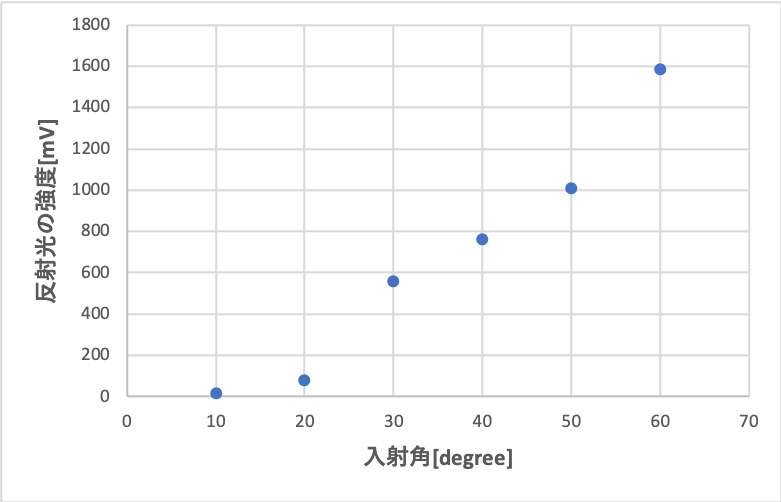
\includegraphics[width=60mm]{fig21.png}
  \end{center}
  \caption{S偏光の反射光強度}
  \label{fig:21}
 \end{minipage}
\end{figure}

表からP偏光では55°付近で反射光強度が著しく低くなる点が存在した。
一方S偏光では反射角が大きくなるにつれて反射光強度は大きくなっていった。

\newpage
\subsubsection{Discussion}
グラフよりP偏光、S偏光どちらも基本的に反射角が大きくなっていくにつれて反射光の強度も強くなっていった。これは入射角の値が大きくなっていくにつれて反射率の値が大きくなっていくためだと考えらえる。
またP偏光においてはブリュースター角付近で反射光の値が非常に小さくなることが確認された。
実験からは$\theta=55°$の時に反射光の値が一番小さくなった。また式(\ref{eq:h})に空中の屈折率1.0,スライドガラスの屈折率1.52を考慮すると、ブリュースター角は$\theta_B=56.659$と計算でき概ね実験結果と同じ値を示した。
しかし実験において56°の値が54°,55°の値よりも大きくなり一つだけ外れた値となってしまった理由としてはフォトディテクターに反射光がまっすぐに当たらなかったことが考えられる。
%=============================================================
%=============================================================
\section{Diffraction grating fabrication by two-beam interference}
\subsection{Diffraction grating fabrication by two-beam interference}
\subsubsection{Purpose}
二つの光によってフォトクロミックプレートに回折格子を生成する。
また生成された回折格子により作られる干渉模様を観測する。
またその干渉縞についての性質を理解する。
\subsubsection{Contents}
図(\ref{fig:22})のように光学系を製作した。
まず偏光板を光路に挿入して光の強度を下げておいた。
偏光された光を50\%のビームスプリッターによってビームを二つに分けた。
分けたビームをそれぞれミラーで反射させてフォトクロミックプレートで一点に集まるように調節した。
この時分けられた光のそれぞれの光路を$Path1=BS - M2 - filter holder$,$Path2=BS - M1 - M3 - filter holder$とする。
光の干渉により回折格子を作りたいのでこのPath1,Path2の光路差がコヒーレント長を上回らないように注意した。
今回の実験での光路長は$Path1=74cm$,$Path2=74cm$であり光路差は0cmとなった。
また二光のなす角$2\theta$が30°を超えないように注意してフィルターホルダー、ミラーの位置を調節した。
今回は$2\theta = 27.7°$とした。
次に偏光板を回し光の強度が強くなるように調節した。
その後フォトクロミックプレートに干渉光を当てることで回折格子をフォトクロミックプレート上に作り出した。
その後フィルターホルダーの後ろに紙をスクリーンとして置き干渉光を観察した。
またPath1,Path2の光を交互に隠すことでスクリーンにどのような干渉スポットが浮かび上がるのかを確認した。

\begin{figure}[htbp]
 \begin{center}
  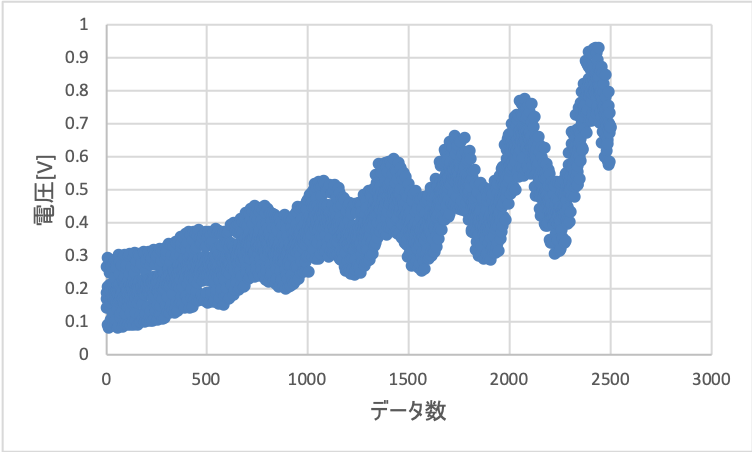
\includegraphics[width=100mm]{fig22.png}
 \end{center}
 \caption{二光干渉による回折格子作成の実験}
 \label{fig:22}
\end{figure}

その次にレーザー光を十分に当てたフォトクロミックプレートを顕微鏡で観察し単位長さあたりに何本の干渉縞が存在しているのかを観察した。

\subsubsection{Result}
偏光板を回転させ光の強度を上げてしばらくフォトクロミックプレートに光を当てるとスクリーン上に干渉スッポットが現れた。
また光路Path1,Path2のどちらを隠しても干渉スッポットは消えることなく存在し続けた。
その後Path2からのビーム光を遮りPath1からの光を用いてスクリーン上の干渉スポットを観察した。
ビーム光の回折格子への入射角は0°,回折角は27.512°であった。
さらにフォトクロミックプレート上には80μmに58本の干渉縞が観察された。

\subsubsection{Discussion}
まずフィルターホルダーの後ろのスクリーンに干渉スポットが観察されたのはフォトクロミックプレート上に干渉模様がうつされたことにより干渉縞の部分のみ光が透過できるようになりフォトクロミックプレートが回折格子の役割を果たしたためだと考えれる。
また、フォトクロミックプレート上に80μmに58本の干渉縞が観察されたことからこの回折格子定数は$d = 1379μm$であることがわかる。
また回折格子の関係式$\lambda = 2dsin\theta$,さらにHe-Neレーザーの波長($\lambda = 632.8\mu m$)と実験より$2 \theta = 27.7$から格子定数$d =1321.79μm$と計算できる。

以上より回折格子定数の実験値と理論値は概ね一致した。
しかし$\theta$の値が大きかったために回折格子定数が小さくり目測で80μmの中に何本の干渉縞があるのかを観察するのが困難になってしまったために理論値に多少の誤差が生じてしまったことなどが考えられる。

またスクリーン上に映った回折光は一つしか観察されなかったのでm = -1,入射角$\theta_1 = 0°$として回折格子の干渉条件
$dsin\theta_1 - dsin\theta_2 = m\lambda$ の関係式に代入して回折角を求めると、$\theta_2 = 27.316$であり実験で計測した27.512°と近い値となった。
この時回折格子に対して入射角が完全に垂直ではなかったことなどが値が異なった理由として考えられる。
 %=============================================================
 %=============================================================
 \section{Holography - two-beam transmission hologram}
 \subsection{Two-beam transmission holograms}
 \subsubsection{Purpose}
 前回の二光干渉による回折格子の製作の原理を用いてホログラムを作る。
 ホログラムの原理を理解する。
 \subsubsection{Contents}
 以下のように光学系を製作する。

 \begin{figure}[htbp]
  \begin{center}
   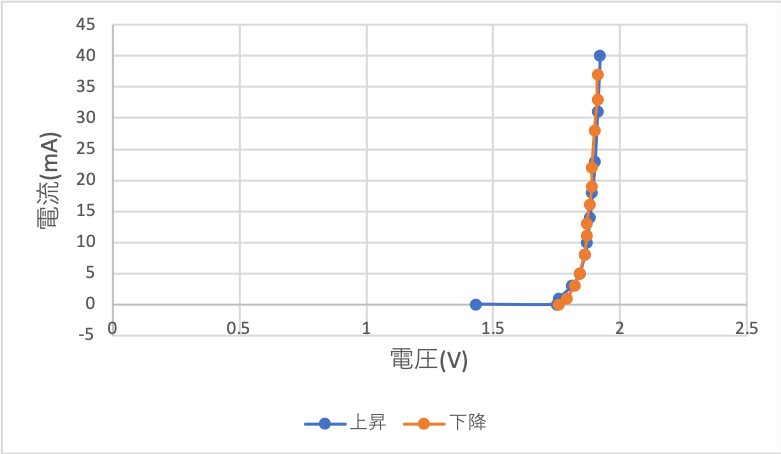
\includegraphics[width=100mm]{fig23.png}
  \end{center}
  \caption{二光干渉によるホログラムの実験}
  \label{fig:23}
 \end{figure}

 まず今回は5\%のビームスプリッターを使用した。また分けたそれぞれの光をL1,L2のレンズによって拡大した。L1によって拡大された光を物体にあて反射光がプレートホルダーに届くように調節した。この時Objectとして白鳥のモデルを使用した。
 また前回から基本的に実験機材を動かしていないため二つの光路差は0となっておりコヒーレント長を上回らないことを確認した。
 またプレートホルダー上において参照光の強度がと物体光の強度が2から3倍となるように計測器を用いて調節した。

 この時参照光強度は0.55μW,物体光強度は0.20μWであった。
 以上結果よりフィルムプレートに露光する時間を計算する。
 ホログラムを作るのに最適な露光時間は$90[\mu J/cm^2]$であるので計測器の面積が$16\pi [mm^2]$であることに注意すると露光時間は60.32[s]と計算できる。

 露光が終わったら次は現像作業を行う。
 現像は以下のような手順で行なった。

 \begin{table}[htb]
   \begin{center}
     \caption{現像の手順}
     \begin{tabular}{|l|l|l|l|} \hline
        項目&&内容&処理時間\\ \hline
        現像&\begin{tabular}{c}現像液\\コピナール\end{tabular}&ホログラム乾板を浸し連続撹拌する&6分\\ \hline
        水洗い&水&水ですすぐ&2分\\ \hline
        定着&\begin{tabular}{c}定着液\\スーパーフィジフィックス\end{tabular}&ホログラム乾板を浸し連続撹拌する&5分\\ \hline
        予備水洗い&水&水ですすぐ&2分\\ \hline
        水洗促進浴&\begin{tabular}{c}水洗促進剤\\フジQW\end{tabular}&浸しながら撹拌する&1分\\ \hline
        水洗い&水&水ですすぐ&2分\\ \hline
        脱水&\begin{tabular}{c}仕上げ剤\\ドライウェル\end{tabular}&浸しながら撹拌する&1分\\ \hline
        乾燥&ドライヤー&ドライヤーの弱冷風を当てる&乾くまで\\ \hline
     \end{tabular}
     \label{tab:1}
   \end{center}
 \end{table}

現像後5\%ビームスプリッターを100\%ビームスプリッターに取り替え参照光を現像したフィルターにあてフィルター越しに干渉光を覗き込んでホログラムが作られているかを確認する。
 \subsubsection{Result}
 現像したフィルターに参照光を当て覗き込むと下の写真のような像が観察できた。
 またこの像は写真などとは異なり三次元的に映し出されていた。

 \begin{figure}[htbp]
  \begin{center}
   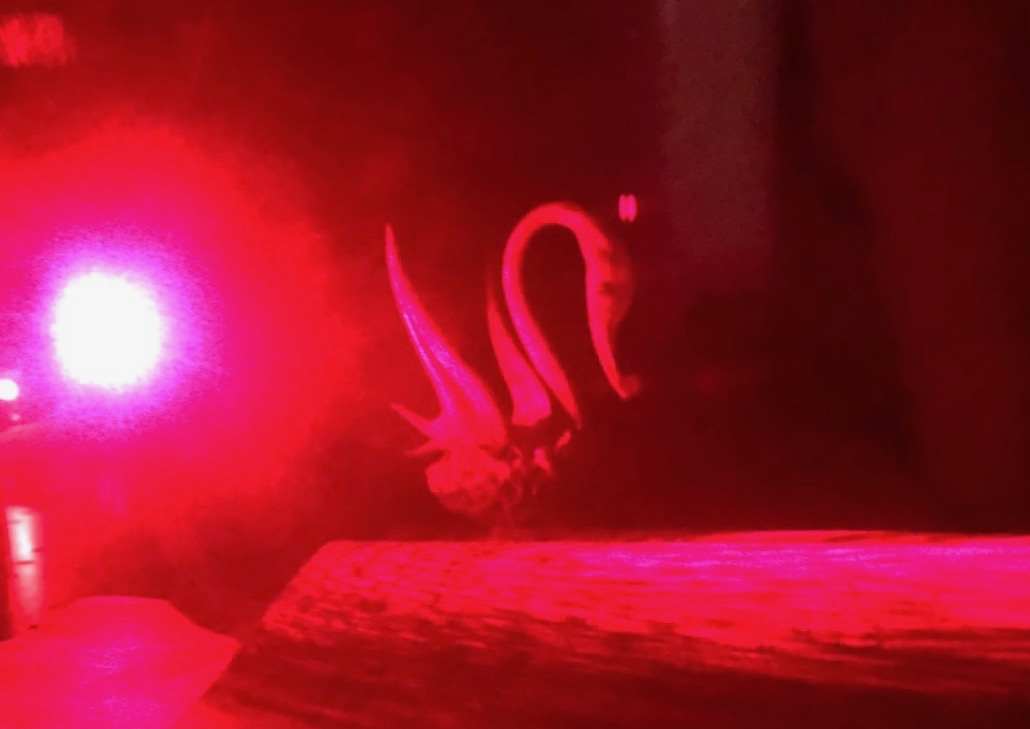
\includegraphics[width=100mm]{fig24.png}
  \end{center}
  \caption{白鳥のホログラム}
  \label{fig:24}
 \end{figure}
\newpage
 \subsubsection{Discussion}
 まず、今回はコヒーレント長を上回らなっかたためにしっかりフィルター上にホログラムを作る回折格子が作られたと考えられる。
 また今回の実験で得られたフィルターが割れたとしてもその破片に同じように参照光を同じ角度で当てるとこのホログラムは再現されると予想される。
 これはホログラムが再生されるためのフィルター上の回折格子の間隔は前回の実験から分かるように数μmのオーダーであるからである。
 そのためある程度小さくプレートを割ったとしてもホログラムが再生されることが予想される。

 またホログラムが作られる原理は参照光をプレートに照射した際に透過光の複素振幅が物体光に比例する光が再生されるためだと説明できる。
% \end{multicols}
\begin{thebibliography}{99}
  \bibitem{光物理学} 櫛田孝司『光物理学』(共立出版,1983)
\end{thebibliography}

\end{document}
